\documentclass[12pt]{article}
\usepackage{geometry}                % See geometry.pdf to learn the layout options. There are lots.
\geometry{letterpaper}                   % ... or a4paper or a5paper or ... 
%\geometry{landscape}                % Activate for for rotated page geometry
\usepackage[parfill]{parskip}    % Activate to begin paragraphs with an empty line rather than an indent
\usepackage{daves,fancyhdr,natbib,graphicx,dcolumn,amsmath,lastpage,url}
\usepackage{amsmath,amssymb,epstopdf,longtable}
\usepackage[final]{pdfpages}
\DeclareGraphicsRule{.tif}{png}{.png}{`convert #1 `dirname #1`/`basename #1 .tif`.png}
\pagestyle{fancy}
\lhead{CE 5364 -- Groundwater Transport Phenomena }
\rhead{FALL 2025}
\lfoot{ES2}
\cfoot{}
\rfoot{Page \thepage\ of \pageref{LastPage}}
\renewcommand\headrulewidth{0pt}



\begin{document}
\begin{center}
{\textbf{{ CE 5364 Groundwater Transport Phenomena } \\ {Exercise Set 3}}}
\end{center}

\section*{\small{Exercises}}
\begin{enumerate} %% Problem Counter

%%%%%%%%%%%%%%%%%%%%%%%%%%%%%%%%%%%%%%%%%%%%%%%%%%%%

\item Figure \ref{fig:site_map_homework1} depicts the general area where the \textsl{Spill-O-Rama} industrial manufacturing plant operates, among other things \textsl{Spill-O-Rama} manufactures titanium knee replacements, using proprietary techniques. The golf course is about 5000 meters west of the plant boundary. The golf course opened about 1980, around the same time as the plant began operations. 

\begin{figure}[h!] %  figure placement: here, top, bottom, or page
   \centering
   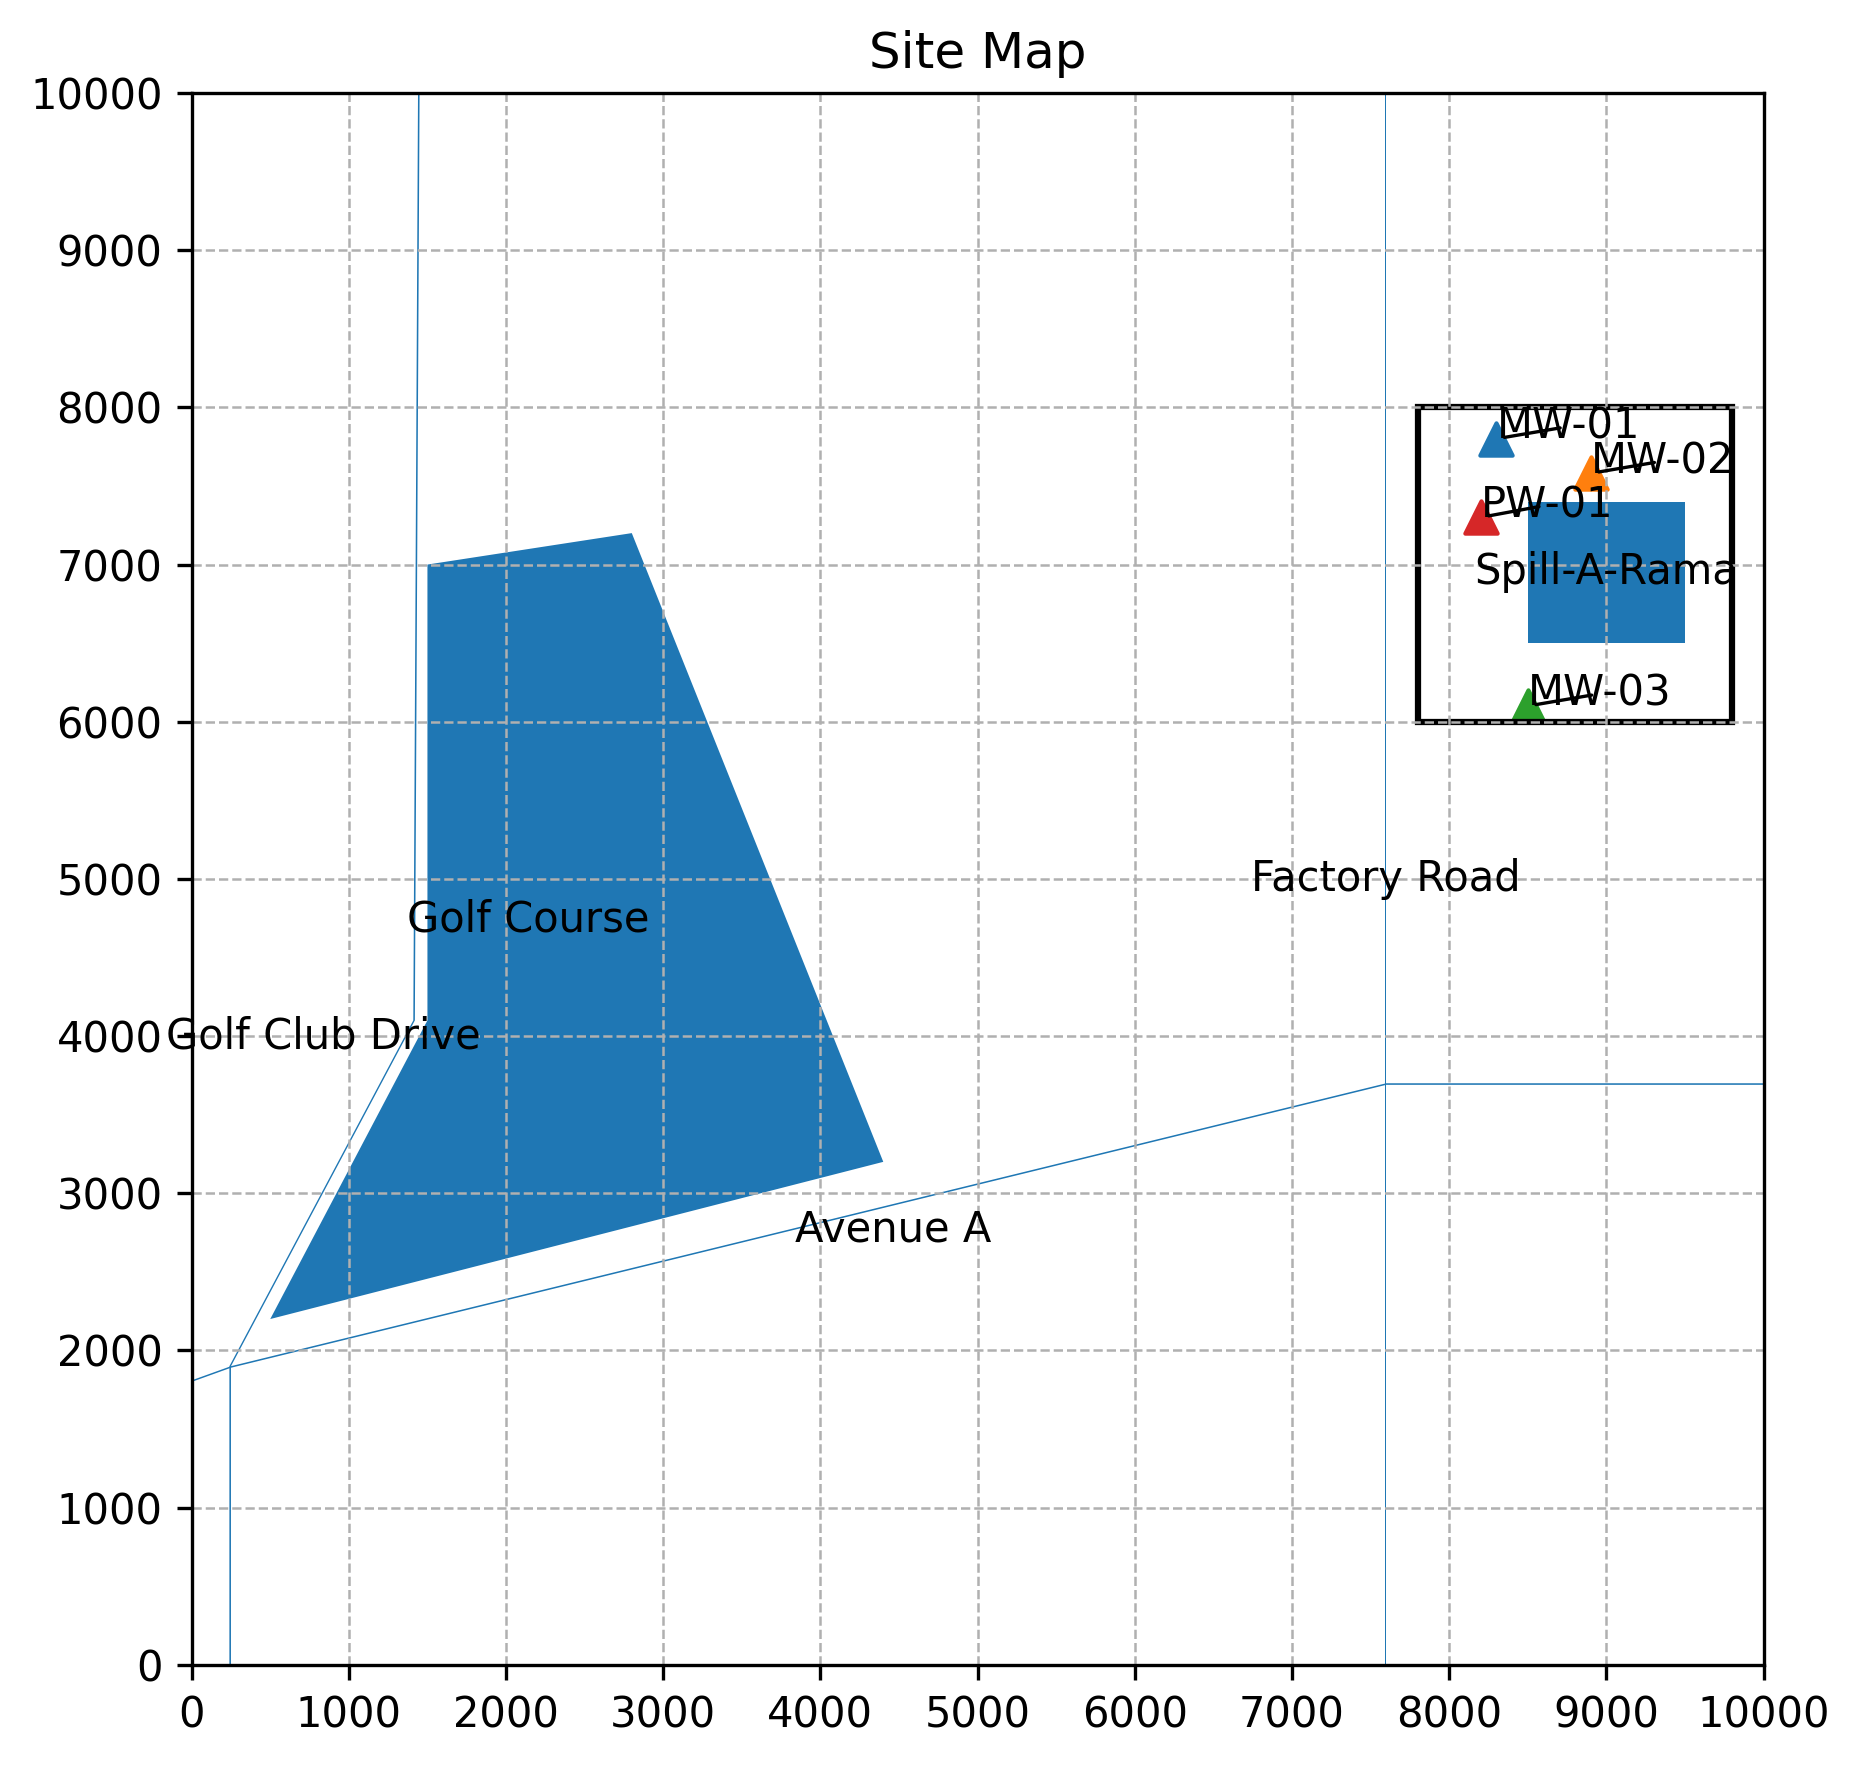
\includegraphics[width=6in]{site_map_homework1.png} 
   \caption{Overview map of the Spill-O-Rama plant and adjacent areas}
   \label{fig:site_map_homework1}
\end{figure}

Figure \ref{fig:site_map_homework2} is a detail map of the plant itself showing the locations of monitoring wells (MW) and a pumping well (PW).

\begin{figure}[h!] %  figure placement: here, top, bottom, or page
   \centering
   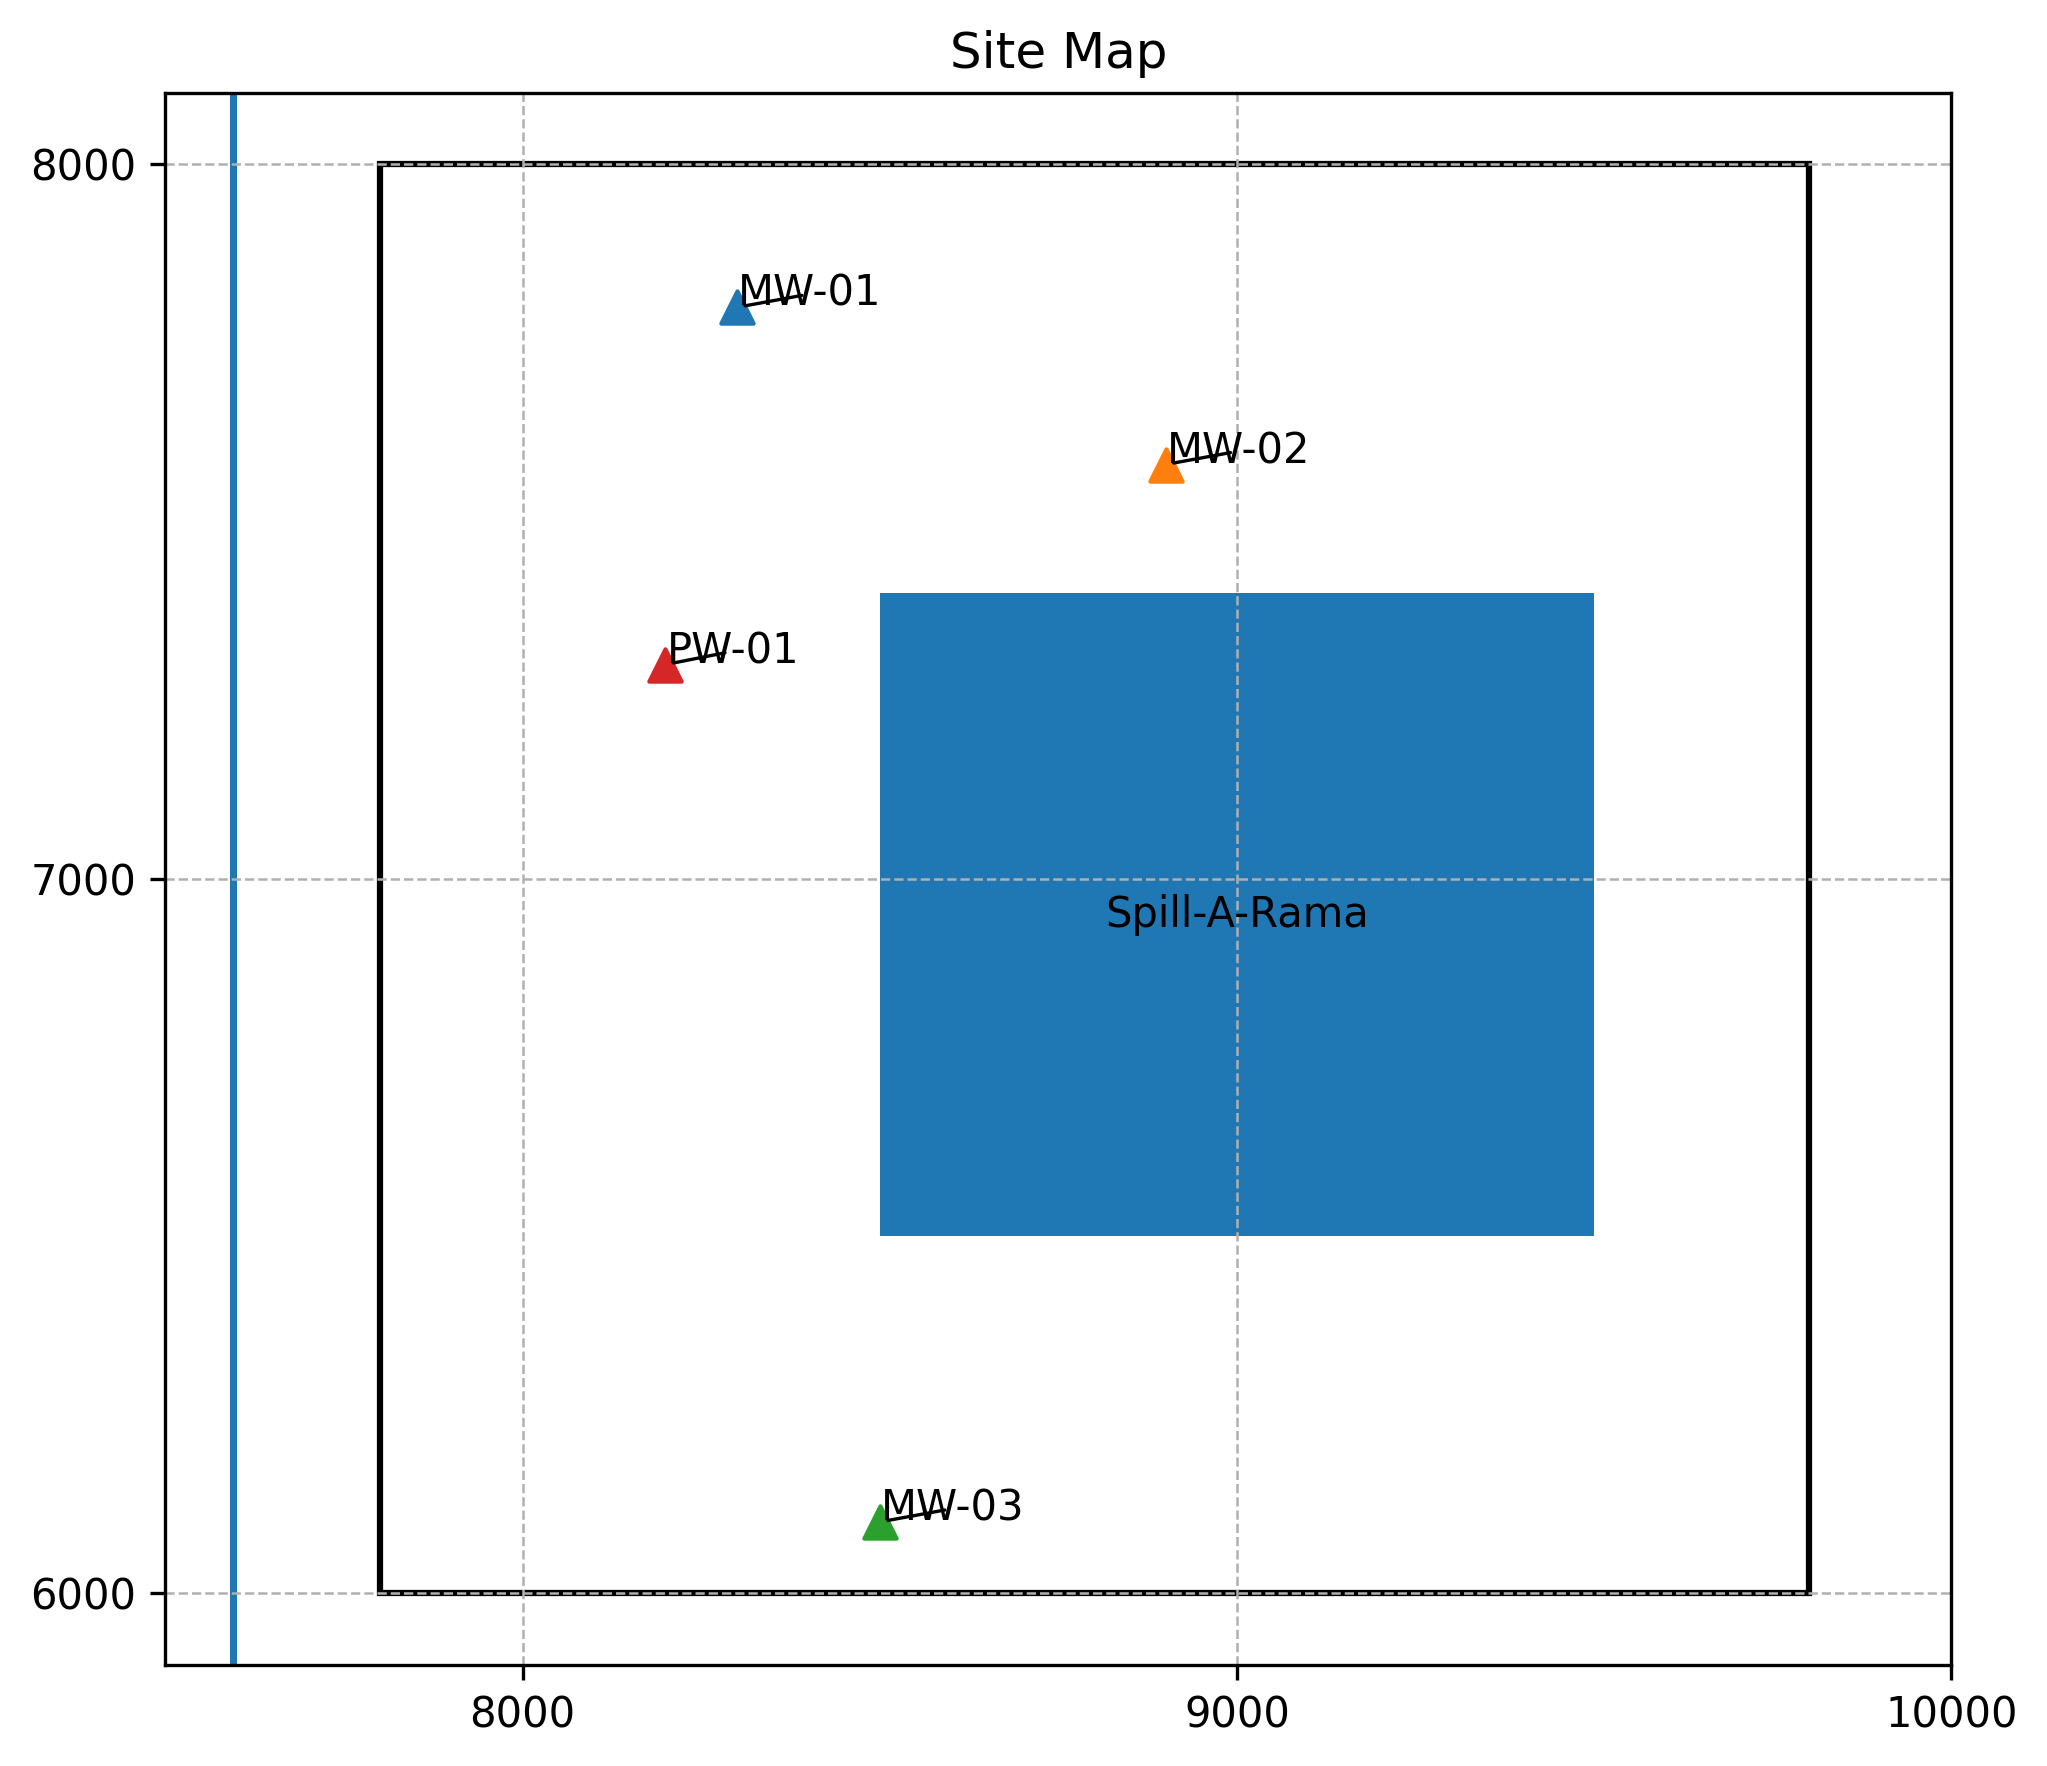
\includegraphics[width=6in]{site_map_homework2.png} 
   \caption{Detail map of the Spill-O-Rama}
   \label{fig:site_map_homework2}
\end{figure}

\clearpage
Figure \ref{fig:drillinglogs} are interpreted borehole logs made by the driller when the monitoring wells were installed.

\begin{figure}[h!] %  figure placement: here, top, bottom, or page
   \centering
   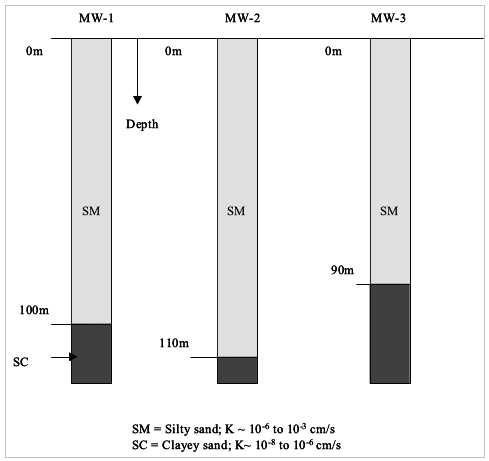
\includegraphics[width=3in]{drillinglogs.png} 
   \caption{MW1, MW2, and MW3 drilling logs}
   \label{fig:drillinglogs}
\end{figure}

The pumping well was installed (PW-1) to provide process and cooling water for the plant. During development of the well a pumping test was conducted and the data from that test are tabulated below.

\begin{table}[h!]
\centering
\caption{Drawdown-Time for 100 gpm pumping at PW1}
\begin{tabular}{lrrr}
~&~&~&~\\
\hline
Time (min) & MW-1 (m) & MW-2 (m) & MW-3 (m) \\
\hline
1.0 & 0.0 & 0.0 & 0.0 \\
6.0 & 0.02 & 0.001 & 0.0 \\
12.0 & 0.096 & 0.015 & 0.0 \\
18.0 & 0.18 & 0.045 & 0.001 \\
24.0 & 0.257 & 0.082 & 0.005 \\
30.0 & 0.326 & 0.121 & 0.012 \\
60.0 & 0.582 & 0.298 & 0.071 \\
90.0 & 0.752 & 0.436 & 0.143 \\
120.0 & 0.88 & 0.546 & 0.212 \\
240.0 & 1.202 & 0.84 & 0.433 \\
480.0 & 1.537 & 1.16 & 0.71 \\
\hline
\end{tabular}
\end{table}

Static long-term water levels in the wells are 81.0m, 80.0m, and 85.0m for MW-1, MW-2, and MW-3, respectively.


Determine:

\begin{enumerate} %% Deliverable Counter
\item Estimate the regional groundwater flow direction from the monitoring wells.
\item Is the groundwater flow direction favorable for constituients to move from the golf course to the plant site
\item Estimate the hydraulic conductivity based on the pumping test results.  
\item If the value of hydraulic conductivity from the pumping tests is comparable to the values shown on the drilling logs.
\item Assume the golf course starts using treated wastewater to irrigate. The irrigation scheme produces a concentration in the groundwater of 10000 ppm nitrate (as nitrate).  How long until nitrate is detected in the MW array?
\item Is nitrate damage to the titanium (i.e. embrittlement) a practical concern for \textsl{Spill-O-Rama}? 
\item (Extra Credit) Assume PW1 operates at 100 gpm as specified.  Construct a map of groundwater elevations for the entire study area (Golf Course and \textsl{Spill-O-Rama}).  
\end{enumerate} %% Deliverable Counter


%%%%%%%%%%%%%%%%%%%%%%%%%%%%%%%%%%%%%%%%%%%%%%%%%%%%%%%%%%%%%%%%%%%
\end{enumerate}%% Problem Counter

\end{document}  